\documentclass{article}

% Document extensibility %
%
% Disables native paragraph indentation
\usepackage{parskip} 
%
% Provides further bullet options for lists
\usepackage{enumitem}

% Mathematical symbol and statement packages %
%
% Necessary
\usepackage{amsmath}
\usepackage{amssymb}
%
% Extensive fraction notation
\usepackage{xfrac}
%
% Generic mathematical commands
% Notable: \degree, \celcius
\usepackage{gensymb}
%
% Variable vector notation (arrow above variable)
\usepackage{esvect}
%
% Multiline boxed equations
\usepackage{empheq}
%
% SI Unit
\usepackage{siunitx}
%
% More intuitive arrays/matrices
\usepackage{array}

% Graphic packages %
%
% Diagrams and illustrations
\usepackage{tikz}
\usetikzlibrary{positioning}
%
% Image insertion
\usepackage{graphicx}
%
%
\usepackage{pgffor}

% Document content %
%
% Change title of table of contents
% \renewcommand{\contentsname}{Title}

\title{Homework 6 - Force Dynamics}
\author{Corey Mostero - 2566652}
\date{20 April 2023}

\begin{document}

% Command `\hr` to insert horizontal rules
\newcommand{\hr}{\par\noindent\rule{\textwidth}{0.4pt}}

% Command to box and center math equations
\newcommand{\bc}[1]{
	\begin{equation*}
		\begin{boxed}
			{#1}
		\end{boxed}
	\end{equation*}
}

% Command for single line equations with a condition
\newcommand{\cond}[2]{
	\ifmmode
		{#1} \quad {#2}
	\else
		$$ {#1} \quad {#2} $$
	\fi
}

\maketitle
\newpage

\tableofcontents

\section{Book}

\subsection{5.12}
\begin{align*}
	m & = \SI{125}{\kilogram} \\
	F_\text{thrust} & = \SI{1720}{\newton} \\
	F_\text{ps} & = \SI{15.5}{\newton}
\end{align*}
\begin{enumerate}[label=\textbf{(\alph*)}]
	\item
		\ \\
		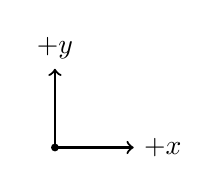
\begin{tikzpicture}
			\node[circle, fill, inner sep = 1pt]{};
			\draw[black, thick, ->] (0, 0) -- (0, 1) node [above] {$ +y $};
			\draw[black, thick, ->] (0, 0) -- (1, 0) node [right] {$ +x $};
		\end{tikzpicture}
		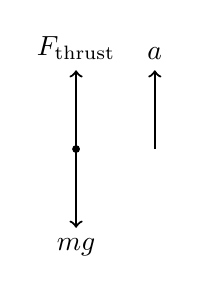
\begin{tikzpicture}
			\node[circle, fill, inner sep = 1pt]{};
			\draw[black, thick, ->] (0, 0) -- (0, 1) node [above] {$ F_\text{thrust} $};
			\draw[black, thick, ->] (0, 0) -- (0, -1) node [below] {$ mg $};
			\draw[black, thick, ->] (1, 0) -- (1, 1) node [above] {$ a $};
		\end{tikzpicture}
		\begin{align*}
			\sum F_y & = ma \\
			F_\text{thrust} & = ma + mg \\
			a & = \frac{F_\text{thrust} - mg}{m} \\
			a & = \frac{\SI{1720}{\newton} - (\SI{125}{\kilogram})(\SI{10}{\meter \per \second \squared})}{\SI{125}{\kilogram}} \\
			a & = \SI{3.76}{\meter \per \second \squared}
		\end{align*}
		\bc{a = \SI{3.76}{\meter \per \second \squared}}
	\item
		\ \\
		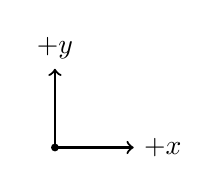
\begin{tikzpicture}
			\node[circle, fill, inner sep = 1pt]{};
			\draw[black, thick, ->] (0, 0) -- (0, 1) node [above] {$ +y $};
			\draw[black, thick, ->] (0, 0) -- (1, 0) node [right] {$ +x $};
		\end{tikzpicture}
		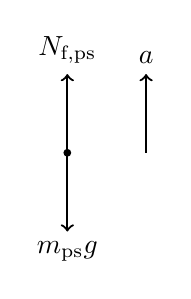
\begin{tikzpicture}
			\node[circle, fill, inner sep = 1pt]{};
			\draw[black, thick, ->] (0, 0) -- (0, 1) node [above] {$ N_\text{f,ps} $};
			\draw[black, thick, ->] (0, 0) -- (0, -1) node [below] {$ m_\text{ps}g $};
			\draw[black, thick, ->] (1, 0) -- (1, 1) node [above] {$ a $};
		\end{tikzpicture}
		\begin{align*}
			\sum F_y & = m_\text{ps}a \\
			N_\text{f,ps} - m_\text{ps}g & = m_\text{ps}a \\
			N_\text{f,ps} & = m_\text{ps}(g + a) \\
			N_\text{f,ps} & = \left( \frac{F_\text{ps}}{g} \right)(g + a) \\
			N_\text{f,ps} & = \left( \frac{\SI{15.5}{\newton}}{\SI{10}{\meter \per \second \squared}} \right) (\SI{10}{\meter \per \second \squared} + \SI{3.76}{\meter \per \second \squared}) \\
			N_\text{f,ps} & = \SI{21.33}{\newton}
		\end{align*}
		\bc{N_\text{f,ps} = \SI{21.33}{\newton}}
\end{enumerate}

\subsection{5.17}
\begin{align*}
	m_1 & = \SI{4.70}{\kilogram} \\
	\mu & = 0 \\
	m_2 & = ? \\
	T & = \SI{13.6}{\newton}
\end{align*}
\begin{enumerate}[label=\textbf{(\alph*)}]
	\item
		\ \\
		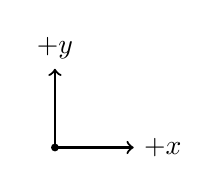
\begin{tikzpicture}
			\node[circle, fill, inner sep = 1pt]{};
			\draw[black, thick, ->] (0, 0) -- (0, 1) node [above] {$ +y $};
			\draw[black, thick, ->] (0, 0) -- (1, 0) node [right] {$ +x $};
		\end{tikzpicture}

		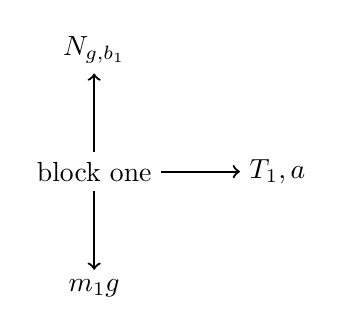
\begin{tikzpicture}
			\node (blockone) {block one};
			\node (normal) [above = of blockone] {$ N_{g,b_1} $};
			\node (weight) [below = of blockone] {$ m_1g $};
			\node (tension) [right = of blockone] {$ T_1, a $};

			\draw[black, thick, ->] (blockone.north) -- (normal.south);
			\draw[black, thick, ->] (blockone.south) -- (weight.north);
			\draw[black, thick, ->] (blockone.east) -- (tension.west);
		\end{tikzpicture} \hspace{1cm}
		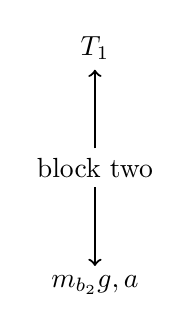
\begin{tikzpicture}
			\node (blocktwo) {block two};
			\node (tension) [above = of blocktwo] {$ T_1 $};
			\node (weight) [below = of blocktwo] {$ m_{b_2}g, a $};

			\draw[black, thick, ->] (blocktwo.north) -- (tension.south);
			\draw[black, thick, ->] (blocktwo.south) -- (weight.north);
		\end{tikzpicture}
	\item
		\begin{align*}
			\sum F_x^{(b_1)} & = m_{b_1}a \\
			T_1 & = m_{b_1}a \\
			a & = \frac{T_1}{m_{b_1}} \\
			a & = \frac{\SI{13.6}{\newton}}{\SI{4.70}{\kilogram}} \\
			a & = \SI{2.89}{\meter \per \second \squared}
		\end{align*}
		\bc{a = \SI{2.89}{\meter \per \second \squared}}
	\item
		\begin{align*}
			\sum F_y^{(b_2)} & = -m_{b_2}a \\
			T_1 - m_{b_2}g & = -m_{b_2}a \\
			m_{b_2} \left( -a + g \right) & = T_1 \\
			m_{b_2} & = \frac{T_1}{-a + g} \\
			m_{b_2} & = \frac{\SI{13.6}{\newton}}{-(\SI{2.89}{\meter \per \second \squared}) + \SI{10}{\meter \per \second \squared}} \\
			m_{b_2} & = \SI{1.91}{\kilogram}
		\end{align*}
		\bc{m_{b_2} = \SI{1.91}{\kilogram}}
	\item
		The weight of the hanging block ($ w_{b_2} $) can be calculated using
		$$ w_{b_2} = m_{b_2}g, $$
		solved as so:
		\begin{align*}
			w_{b_2} & = m_{b_2}g \\
					& = (\SI{1.91}{\kilogram})(\SI{10}{\meter \per \second \squared}) \\
			w_{b_2} & = \SI{19.1}{\newton}
		\end{align*}
		\bc{\therefore \text{ it can be shown that } w_{b_2} > T_1}
\end{enumerate}

\subsection{5.21}
\begin{align*}
	m & = \SI{2.10}{\kilogram} \\
	v & = \SI{8.50}{\meter \per \second} \\
	t & = 0 \\
	F(t) & = (\SI{6.00}{\newton \per \second \squared})t^2
\end{align*}
\begin{enumerate}[label=\textbf{(\alph*)}]
	\item
		Using the force function and NSL, solve for the acceleration function and integrate to get the velocity function.
		\begin{align*}
			F(t) & = ma \\
			a(t) & = \frac{F}{m} \\
			a(t) & = \frac{-\SI{6.00}{\newton \per \second \squared}}{\SI{2.10}{\kilogram}}t^2 \\
			a(t) & = (-\SI{2.86}{\meter \per \second \tothe 4})t^2
		\end{align*}
		\begin{align*}
			v(t) & = \int a(t) dt = \int (-\SI{2.86}{\meter \per \second \tothe 4})t^2 dt \\
			v(t) & = (-\SI{0.953}{\meter \per \second \tothe 4})t^3 + v \\
			v(t) & = (-\SI{0.953}{\meter \per \second \tothe 4})t^3 + \SI{8.50}{\meter \per \second}
		\end{align*}
		Find $ t $ when the velocity is $ 0 $.
		\begin{align*}
			v(t) & = (-\SI{0.953}{\meter \per \second \tothe 4})t^3 + \SI{8.50}{\meter \per \second} = 0 \\
			(\SI{0.953}{\meter \per \second \tothe 4})t^3 & = \SI{8.50}{\meter \per \second} \\
			t & = \SI{2.07}{\second}
		\end{align*}
		Integrate and find the distance at time, $ t = \SI{2.07}{\second} $.
		\begin{align*}
			x(t) & = \int v(t) dt = \int (-\SI{0.953}{\meter \per \second \tothe 4})t^3 + \SI{8.50}{\meter \per \second} dt \\
			x(t) & = (-\SI{0.238}{\meter \per \second \squared})t^4 + (\SI{8.50}{\meter \per \second})t + 0
		\end{align*}
		\begin{align*}
			x(\SI{2.07}{\second}) & = (-\SI{0.238}{\meter \per \second \squared})(\SI{2.07}{\second})^4 + (\SI{8.50}{\meter \per \second})(\SI{2.07}{\second}) \\
			x(\SI{2.07}{\second}) & = \SI{13.2}{\meter}
		\end{align*}
		\bc{x = \SI{13.2}{\meter}}
	\item
		Find $ v $ at time $ t = \SI{3.00}{\second} $.
		\begin{align*}
			v(\SI{3.00}{\second}) & = (-\SI{0.953}{\meter \per \second \tothe 4})(\SI{3.00}{\second})^3 + \SI{8.50}{\meter \per \second} \\
			v(\SI{3.00}{\second}) & = -\SI{17.2}{\meter \per \second}
		\end{align*}
		\bc{v = -\SI{17.2}{\meter \per \second}}
\end{enumerate}

\subsection{5.33}
\begin{align*}
	m_\text{top} & = \SI{32.0}{\kilogram} \\
	m_\text{bottom} & = \SI{48.0}{\kilogram} \\
	\Delta y & = \SI{2.50}{\meter} \\
	\Delta x & = \SI{4.75}{\meter} \\
	v & = \SI{15.0}{\centi \meter \per \second} \\
	\mu_k & = 0.444 \\
	\mu_s & = 0.800 \\
	a_x & = 0 \text{ (constant)}
\end{align*}
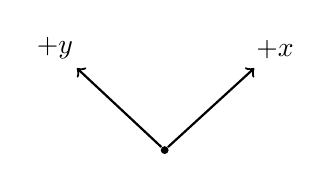
\begin{tikzpicture}
	\node[circle, fill, inner sep = 1pt] (origin) {};
	\node (y) [above left = of origin] {$ +y $};
	\node (x) [above right = of origin] {$ +x $};

	\draw[black, thick, ->] (origin) -- (y);
	\draw[black, thick, ->] (origin) -- (x);
\end{tikzpicture}

\begin{tikzpicture}
	\node (top) {top};
	\node (normal) [above left = of top] {$ N_{\text{bottom, top}} $};
	\node (weight) [below = of top] {$ m_{\text{top}}g $};
	\node (friction) [above right = of top] {$ f_s, a $};

	\foreach \node in {normal, weight, friction}
		\draw[black, thick, ->] (top) -- (\node);
\end{tikzpicture}

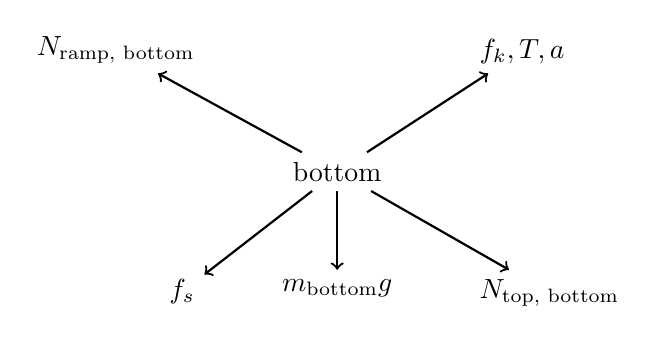
\begin{tikzpicture}
	\node (bottom) {bottom};
	\node (normal_top) [below right = of bottom] {$ N_{\text{top, bottom}} $};
	\node (normal_ramp) [above left = of bottom] {$ N_{\text{ramp, bottom}} $};
	\node (weight) [below = of bottom] {$ m_{\text{bottom}}g $};
	\node (acceleration) [below left = of bottom] {$ f_s $};
	\node (friction) [above right = of bottom] {$ f_k, T, a $};

	\foreach \node in {normal_top, normal_ramp, weight, acceleration, friction}
		\draw[black, thick, ->] (bottom) -- (\node);
\end{tikzpicture}
\begin{enumerate}[label=\textbf{(\alph*)}]
	\item
		\begin{align*}
			\tan(\theta) & = \frac{y}{x} \\
			\theta & = \arctan \left( \frac{y}{x} \right) \\
			\theta & = \arctan \left( \frac{\SI{2.50}{\meter}}{\SI{4.75}{\meter}} \right) \\
			\theta & = \SI{27.8}{\degree}
		\end{align*}
		\begin{align*}
			\sum F_y^{(\text{t, b})} & = m_\text{t, b}g\cos(\SI{27.8}{\degree}) \\
			N_\text{b, t} - N_\text{t, b} + N_\text{r, b} & = m_\text{t, b}g\cos(\SI{27.8}{\degree}) \\
			N_\text{r, b} & = m_\text{t, b}g\cos(\SI{27.8}{\degree}) \\
			N_\text{r, b} & = (\SI{32.0}{\kilogram} + \SI{48.0}{\kilogram})(\SI{10}{\meter \per \second \squared})\cos(\SI{27.8}{\degree}) \\
			N_\text{r, b} & = \SI{707.7}{\newton}
		\end{align*}
		\begin{align*}
			\sum F_x^{(\text{t, b})} & = m_\text{t, b}a \\
			f_s - f_s + f_k + T - m_\text{t, b}g\sin(\SI{27.8}{\degree}) & = (m_\text{t, b})(0) \\
			\mu_kN_\text{r, b} + T - m_\text{t, b}g\sin(\SI{27.8}{\degree}) & = 0 \\
			T & = m_\text{t, b}g\sin(\SI{27.8}{\degree}) - \mu_kN_\text{r, b} \\
			T & = (\SI{32.0}{\kilogram} + \SI{48.0}{\kilogram})(\SI{10}{\meter \per \second \squared})\sin(\SI{27.8}{\degree}) - (0.444)(\SI{707.7}{\newton}) \\
			T & = \SI{58.9}{\newton}
		\end{align*}
		\bc{T = \SI{58.9}{\newton}}
	\item
		\begin{align*}
			\sum F_x^{(\text{top})} & = 0 \\
			f_s & = m_\text{top}g\sin(\SI{27.8}{\degree}) \\
			f_s & = (\SI{32.0}{\kilogram})(\SI{10.0}{\meter \per \second \squared})\sin(\SI{27.8}{\degree}) \\
			f_s & = \SI{149.2}{\newton}
		\end{align*}
		\bc{f_s = \SI{149.2}{\newton} \text { at } \theta = \SI{27.8}{\degree}}
\end{enumerate}

\subsection{5.34}
\begin{align*}
	w_A & = \SI{45.0}{\newton} \\
	w_B & = \SI{25.0}{\newton} \\
	a_B & = 0
\end{align*}
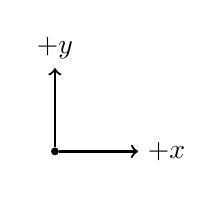
\begin{tikzpicture}
	\node [circle, fill, inner sep = 1pt] (origin) {};
	\node (y) [above = of origin] {$ +y $};
	\node (x) [right = of origin] {$ +x $};

	\foreach \node in {y, x}
		\draw[black, thick, ->] (origin) -- (\node);
\end{tikzpicture}

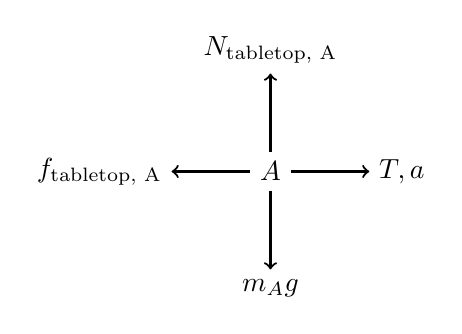
\begin{tikzpicture}
	\node (origin) {$ A $};
	\node (above) [above = of origin] {$ N_\text{tabletop, A} $};
	\node (right) [right = of origin] {$ T, a $};
	\node (below) [below = of origin] {$ m_Ag $};
	\node (left) [left = of origin] {$ f_\text{tabletop, A} $};

	\foreach \node in {above, right, below, left}
		\draw[black, thick, ->] (origin) -- (\node);
\end{tikzpicture} \hspace{1cm}
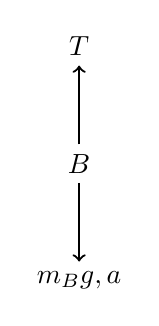
\begin{tikzpicture}
	\node (origin) {$ B $};
	\node (above) [above = of origin] {$ T $};
	\node (below) [below = of origin] {$ m_Bg, a $};

	\foreach \node in {above, below}
		\draw[black, thick, ->] (origin) -- (\node);
\end{tikzpicture}
\begin{enumerate}[label=\textbf{(\alph*)}]
	\item
		\begin{align*}
			w_A & = m_Ag \\
			m_A & = \frac{w_A}{g} \\
			m_A & = \frac{\SI{45.0}{\newton}}{\SI{10}{\meter \per \second \squared}} \\
			m_A & = \SI{4.5}{\kilogram}
		\end{align*}
		\begin{align*}
			w_B & = m_Bg \\
			m_B & = \frac{w_B}{g} \\
			m_B & = \frac{\SI{25.0}{\newton}}{\SI{10}{\meter \per \second \squared}} \\
			m_B & = \SI{2.5}{\kilogram}
		\end{align*}
		\begin{align*}
			\sum F_y^{(B)} & = -m_Ba \\
			T - m_Bg & = (-m_B)(0) \\
			T & = m_Bg \\
			T & = \SI{25.0}{\newton}
		\end{align*}
		\begin{align*}
			\sum F_y^{(A)} & = 0 \\
			N_\text{t, A} & = m_Ag \\
			N_\text{t, A} & = \SI{45.0}{\newton}
		\end{align*}
		\begin{align*}
			\sum F_x^{(A)} & = m_Aa \\
			T - \mu N_\text{t, A} & = (m_A)(0) \\
			\mu & = \frac{T}{N_\text{t, A}} \\
			\mu & = \frac{\SI{25.0}{\newton}}{\SI{45.0}{\newton}} \\
			\mu & = 0.556
		\end{align*}
		\bc{\mu = 0.556}
	\item
		\begin{align*}
			\sum F_y^{(A)} & = 0 \\
			N_\text{t, A} - m_Ag & = 0 \\
			N_\text{t, A} & = m_Ag \\
			N_\text{t, A} & = 2(\SI{45.0}{\newton}) \\
			N_\text{t, A} & = \SI{90.0}{\newton}
		\end{align*}
		\begin{align*}
			\sum F_x^{(A)} & = m_Aa \\
			T - f_\text{t, A} & = m_Aa \\
			T & = \mu N_\text{t, A} + m_Aa
		\end{align*}
		\begin{align*}
			w_A & = m_Ag \\
			m_A & = \frac{\SI{90.0}{\newton}}{\SI{10.0}{\meter \per \second \squared}} \\
			m_A & = \SI{9.00}{\kilogram}
		\end{align*}
		\begin{align*}
			\sum F_y^{(B)} & = -m_Ba \\
			T - m_Bg & = -m_Ba \\
			(\mu N_\text{t, A} + m_Aa) - m_Bg & = -m_Ba \\
			-m_Aa - m_Ba & = \mu N_\text{t, A} - m_Bg \\
			a & = \frac{\mu N_\text{t, A} - m_Bg}{-m_A - m_B} \\
			a & = \frac{(0.556)(\SI{90.0}{\newton}) - \SI{25.0}{\newton}}{-(\SI{9.00}{\kilogram}) - \SI{2.5}{\kilogram}} \\
			a & = \SI{-2.18}{\meter \per \second \squared}
		\end{align*}
		\bc{a = \SI{-2.18}{\meter \per \second \squared}}
\end{enumerate}

\section{Lab Manual}

\subsection{571}
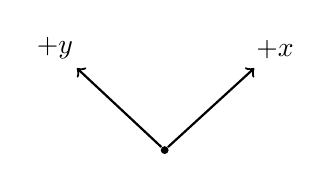
\begin{tikzpicture}
	\node[circle, fill, inner sep = 1pt] (origin) {};
	\node (y) [above left = of origin] {$ +y $};
	\node (x) [above right = of origin] {$ +x $};

	\foreach \node in {y, x}
		\draw[black, thick, ->] (origin) -- (\node);
\end{tikzpicture}

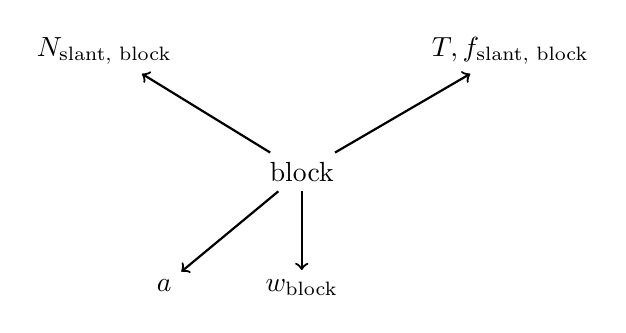
\begin{tikzpicture}
	\node (origin) {block};
	\node (above_right) [above right = of origin] {$ T, f_\text{slant, block} $};
	\node (above_left) [above left = of origin] {$ N_\text{slant, block} $};
	\node (below_left) [below left = of origin] {$ a $};
	\node (below) [below = of origin] {$ w_\text{block} $};

	\foreach \node in {above_right, above_left, below_left, below}
		\draw[black, thick, ->] (origin) -- (\node);
\end{tikzpicture}

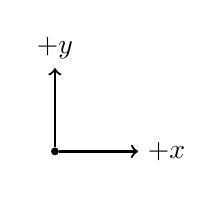
\begin{tikzpicture}
	\node[circle, fill, inner sep = 1pt] (origin) {};
	\node (y) [above = of origin] {$ +y $};
	\node (x) [right = of origin] {$ +x $};

	\foreach \node in {y, x}
		\draw[black, thick, ->] (origin) -- (\node);
\end{tikzpicture}

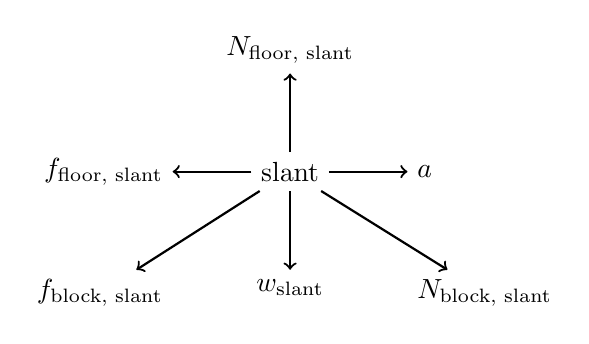
\begin{tikzpicture}
	\node (origin) {slant};
	\node (above) [above = of origin] {$ N_\text{floor, slant} $};
	\node (right) [right = of origin] {$ a $};
	\node (below_right) [below right = of origin] {$ N_\text{block, slant} $};
	\node (below) [below = of origin] {$ w_\text{slant} $};
	\node (below_left) [below left = of origin] {$ f_\text{block, slant} $};
	\node (left) [left = of origin] {$ f_\text{floor, slant} $};

	\foreach \node in {above, right, below_right, below, below_left, left}
		\draw[black, thick, ->] (origin) -- (\node);
\end{tikzpicture}

\begin{align*}
	\sum F_y^{(b)} & = 0 \\
	N_{s, b} - w_b & = 0 \\
	N_{s, b} & = w_b
\end{align*}
\begin{align*}
	\sum F_x^{(b)} & = -m_ba \\
	T + f_{s, b} & = -m_ba \\
	T + \mu N_{s, b} & = -m_ba \\
	a & = -\frac{T + \mu N_{s, b}}{m_b}
\end{align*}

\subsection{575}

\subsection{577}

\subsection{578}

\end{document}
